\section{Guidance-Parameter Optimization Based on BC-TD3}
This section develops a BC-TD3 framework for guidance-parameter optimization to solve \cref{prb:weights}. First, using the structure of the closed-loop guidance law \eqref{eq:48}, the continuous-time parameter optimization problem is transcribed by single shooting into a finite-dimensional nonlinear program (NLP). Expert trajectories that satisfy the minimum evasion distance and the target-arrival accuracy are then generated offline under randomly sampled initial conditions. A BC-TD3 network is constructed next. The actor is pre-trained by behavior cloning on the expert demonstrations, and the demonstrations are used to pre-fill the replay buffer. During subsequent TD3 fine-tuning, a decaying behavior-cloning regularization term is retained in the actor loss, which gradually transfers the policy from expert imitation to reward-driven optimization.

\subsection{Expert-trajectory generation}
In the training scenarios, the simulated initial positions of the NCVs coincide with the target, that is, with the origin of the frame OXYZ. From the geometry, the lead angles of an NCV velocity are

\begin{equation}
\label{eq:67}
\left\{ {\begin{array}{*{20}{l}}
  {{\eta _{yDi}} = {\theta _{Di}} - {q_{yi}}} \\ 
  {{\eta _{zDi}} = {\psi _{{V_{Di}}}} - {q_{zi}}} 
\end{array},{\text{ }}i = 1,2} \right.
\end{equation}
The lead angles of the evader velocity relative to the $i$th NCV are

\begin{equation}
\label{eq:68}
\left\{ {\begin{array}{*{20}{l}}
  {{\eta _{yAi}} = {\theta _A} + {q_{yi}}} \\ 
  {{\eta _{zAi}} = {\psi _{{V_A}}} - {q_{zi}} - \pi } 
\end{array}} \right.
\end{equation}
Taking the main factors that affect evasion effectiveness into account, the initial angular state of the evader relative to the $i$th NCV is defined as ${X_i} = [{q_{yi0}},{q_{zi0}},{\eta _{yAi0}},{\eta _{zAi0}},{\eta _{yDi0}},{\eta _{zDi0}}]$ ($i = 1,2$). In the training samples, when the evader enters an evasive state against one NCV, the difference between the two NCV--evader ranges is set not to exceed 3~km. Let the random variable $\beta  \in [ - 1.5,1.5]{\text{km}}$ be an adjustment variable and ${r_{AD{\text{0}}}}$ the midpoint, with ${r_{AD10}} = {r_{AD0}} + \beta $ and ${r_{AD20}} = {r_{AD0}} - \beta $. The 14-dimensional initial state $X = {[{X_1},{X_2},{r_{AD0}},\beta ]^T}$ is then the initial state of the whole flight, and the four-dimensional guidance-parameter vector ${\mathbf{p}} = {[w,{\kern 1pt} \gamma ,{\kern 1pt} {w_T},{\kern 1pt} {w_E}]^T}$ is the decision variable to be solved by shooting and by reinforcement-learning training.
Single shooting is a direct transcription method for continuous-time optimal control. It is simple to implement and compatible with standard NLP solvers. Unlike collocation, which discretizes the state and the control simultaneously on a dense node set, single shooting parameterizes only the decision variables and recovers the trajectory by forward integration of the system dynamics, converting an infinite-dimensional optimal-control problem into a finite-dimensional parameter optimization problem.

On the engagement interval $[{t_0},{t_f}]$, the guidance-parameter vector ${\mathbf{p}} = {[w,{\kern 1pt} \gamma ,{\kern 1pt} {w_T},{\kern 1pt} {w_E}]^T}$ to be decided is represented by $K$ piecewise-constant segments:

\begin{equation}
\label{eq:69}
{\mathbf{p}}(t) = {{\mathbf{p}}_k},\quad t \in [{t_{k - 1}},{\kern 1pt} {t_k}),\quad k = 1, \ldots ,K
\end{equation}
where $K=10$ and the segment boundaries are equally spaced. The guidance parameter ${\mathbf{p}}$ remains four-dimensional, but only weight ratios act in the closed-loop guidance law. To remove the common scale redundancy of the weights, the total evasion weight is fixed at ${w_k} = w = {10^4}$. The actual decision variables of the shooting method are therefore $[{\gamma _k},{\kern 1pt} {w_{T,k}},{\kern 1pt} {w_{E,k}}]$ on each segment. The resulting expert parameters are further converted into the three-dimensional action labels defined by \eqref{eq:73}. The desired evasion distance is ${d^*} = 20{\kern 1pt} {\text{m}}$.

Given a candidate parameter sequence $\{ {{\mathbf{p}}_k}\} _{k = 1}^K$, the engagement kinematics \eqref{eq:1}--\eqref{eq:5} are integrated forward by the fourth-order Runge--Kutta method (RK4) with step $\Delta t = 0.1{\kern 1pt} {\text{s}}$:

\begin{equation}
\label{eq:70}
X({t_{n + 1}}) = X({t_n}) + \frac{{\Delta t}}{6}({k_1} + 2{k_2} + 2{k_3} + {k_4})
\end{equation}
where $X$ denotes the full system state and ${k_1}, \ldots ,{k_4}$ are the RK4 increments computed from the closed-loop guidance law \eqref{eq:48} under the parameters of the current segment. The NLP objective is constructed from the performance index \eqref{eq:23}:

\begin{equation}
\label{eq:71}
\mathop {\min }\limits_{\{ {{\mathbf{p}}_k}\} _{k = 1}^K} \mathcal{J} = {s_w}\sum\limits_{i = 1}^2 {{{\left[ {d_i^{{\text{actual}}} - {d_i}} \right]}^2}}  + {s_{{w_E}}}\int_{{t_0}}^{{t_f}} {{\mathbf{u}}_A^T{{\mathbf{u}}_A}d\tau }  + {s_{{w_T}}}{\left\| {{r_{AT}}({t_{fT}})} \right\|^2}
\end{equation}
where ${s_w} = 2 \times {10^3}$, ${s_{{w_E}}} = 55$, and ${s_{{w_T}}} = 22$ are fixed scaling coefficients, and $d_i^{{\text{actual}}}$ is the actual minimum approach distance relative to NCV $D_i$. The resulting NLP is solved by IPOPT with an L-BFGS Hessian approximation.

The trajectories obtained by single shooting serve as the expert demonstrations for the subsequent BC-TD3 training. The expert data set is ${\mathcal{D}_{{\text{expert}}}} = \{ {\zeta ^{(1)}},{\kern 1pt} {\zeta ^{(2)}},{\kern 1pt}  \ldots ,{\kern 1pt} {\zeta ^{({N_{{\text{expert}}}})}}\} $, where each trajectory ${\zeta ^{(\ell )}} = \{ ({\mathbf{s}}_n^{(\ell )},{\kern 1pt} {\mathbf{a}}_n^{(\ell )})\} _{n = 1}^{{N_\ell }}$ consists of ${N_\ell}$ state--action pairs extracted from the trajectory. Latin hypercube sampling draws ${N_{{\text{expert}}}} = 2400$ initial conditions in the 14-dimensional initial-state space, which yields about $8$--$15 \times {10^4}$ expert state--action samples.

\subsection{Construction of the BC-TD3 network}
\subsubsection{State space, action space, and reward}
State space (13-dimensional relative engagement state):

\begin{equation}
\label{eq:72}
{\mathbf{s}}(t) = {[\underbrace {{r_{A{D_1}}},{\kern 1pt} {{\dot r}_{A{D_1}}},{\kern 1pt} {q_{{y_1}}},{\kern 1pt} {q_{{z_1}}}}_{{\text{NCV 1}}},\;\underbrace {{r_{A{D_2}}},{\kern 1pt} {{\dot r}_{A{D_2}}},{\kern 1pt} {q_{{y_2}}},{\kern 1pt} {q_{{z_2}}}}_{{\text{NCV 2}}},\;\underbrace {{r_{AT}},{\kern 1pt} {q_\theta },{\kern 1pt} {q_\psi }}_{{\text{Target}}},\;\underbrace {{V_A},{\kern 1pt} \bar{t}_{go}}_{{\text{Evader}}}]^T} \in {\mathbb{R}^{13}}
\end{equation}
where $\bar{t}_{go} = \min ({t_{go,1}},{t_{go,2}})$ is the smaller time-to-go of the two NCVs. This state represents the relative geometry and kinematics of the evader with respect to the two NCVs and the target, and supports the guidance-parameter decision.

Action space (three-dimensional weight combination):

\begin{equation}
\label{eq:73}
{\mathbf{a}}(t) = {[\frac{w}{{{w_E}}},{\kern 1pt} \frac{{{w_T}}}{{{w_E}}},\gamma ]^T} \in {\mathbb{R}^3}
\end{equation}
The guidance parameter ${\mathbf{p}} = {[w,\gamma ,w_T,w_E]^T}$ remains four-dimensional. Because $w$ is fixed, the three action components determine the weight relations required by the closed-loop guidance law. Writing ${\mathbf{a}} = {[a_1,a_2,a_3]^T}$ gives $w_E = w/a_1$, $w_T = a_2w_E$, and $\gamma = a_3$. The meaning of each parameter is given at the end of Section~2.

The reward consists of a stepwise process reward during the evasion phase and a terminal reward settled after the phase-3 PN integral rollout. The process reward is

\begin{equation}
\label{eq:74}
\left\{
\begin{aligned}
& {R_1} = 0.05{\log _{10}}(\min ({r_{AD1}},{d^*}) - 5),if{\text{ }}{r_{AD1,\min }} \geqslant 6{\text{m }}else{\text{ }}0 \\
& {R_2} = 0.05{\log _{10}}(\min ({r_{AD2}},{d^*}) - 5),if{\text{ }}{r_{AD2,\min }} \geqslant 6{\text{m }}else{\text{ }}0
\end{aligned}
\right.
\end{equation}
where $R_1$ and $R_2$ are the process rewards for evading the two NCVs, and ${r_{ADi,\min }} = \min {r_{ADi}}(t)$ is the minimum approach distance to NCV ${D_i}$ over the whole engagement.

The terminal reward is

\begin{equation}
\label{eq:75}
\left\{
\begin{aligned}
& {R_T} = \frac{{80}}{{5 + {r_{AT,end}}}} \\
& {R_{bonus}} = 100,{\text{ }}if{\text{ }}{r_{AT,end}} \leqslant 10{\text{m }}else{\text{ }}0 \\
& {R_{penalty}} =  - 50,{\text{ }}if{\text{ min(}}{r_{AD1,\min }},{r_{AD2,\min }}{\text{)}} \leqslant 6{\text{m }}else{\text{ }}0
\end{aligned}
\right.
\end{equation}
where ${r_{AT,end}}$ is the terminal arrival error at the target obtained by the phase-3 PN rollout, and $R_T$ is the arrival-accuracy reward based on that terminal accuracy. ${R_{bonus}}$ is an additional reward given when evasion and target arrival are both completed, and ${R_{penalty}}$ is an additional penalty given when evasion fails.

\subsubsection{Network architecture}
The BC-TD3 framework uses a two-stage training paradigm: behavior-cloning (BC) pre-training, followed by TD3 reinforcement-learning fine-tuning with decaying BC regularization. Both stages are fully offline.

Actor network ${\pi _\phi }({\mathbf{s}})$: it maps the 13-dimensional state to a 3-dimensional action,

\begin{equation}
\label{eq:76}
{\pi _\phi }({\mathbf{s}}) = {{\mathbf{a}}_{\max }} \cdot \tanh ({{\mathbf{W}}_3}{\kern 1pt} {\text{ReLU}}({{\mathbf{W}}_2}{\kern 1pt} {\text{ReLU}}({{\mathbf{W}}_1}{\mathbf{s}} + {{\mathbf{o}}_1}) + {{\mathbf{o}}_2}) + {{\mathbf{o}}_3})
\end{equation}
The hidden layers are $[256, 256]$ with ReLU activation, and the output layer is $\tanh$ so that the action is bounded. Here ${{\mathbf{o}}_1}$, ${{\mathbf{o}}_2}$, and ${{\mathbf{o}}_3}$ are the bias vectors of the three layers.

Twin critic networks ${Q_{{\psi _1}}}({\mathbf{s}},{\mathbf{a}})$ and ${Q_{{\psi _2}}}({\mathbf{s}},{\mathbf{a}})$: each maps the concatenated pair $({\mathbf{s}},{\mathbf{a}})$ to a scalar Q-value,

\begin{equation}
\label{eq:77}
{Q_{{\psi _j}}}({\mathbf{s}},{\mathbf{a}}) = {\mathbf{W}}_3^{(j)}{\kern 1pt} {\text{ReLU}}({\mathbf{W}}_2^{(j)}{\kern 1pt} {\text{ReLU}}({\mathbf{W}}_1^{(j)}[{\mathbf{s}};{\kern 1pt} {\mathbf{a}}] + {\mathbf{o}}_1^{(j)}) + {\mathbf{o}}_2^{(j)}) + o_3^{(j)},\quad j = 1,2
\end{equation}
The hidden layers are $[256, 256]$ with a linear output. The target networks \(\pi_{\phi'}\), \(Q_{\psi_1'}\), and \(Q_{\psi_2'}\) are maintained by soft copies to stabilize training.

For BC pre-training, the actor is first trained by supervised behavior cloning on the expert data set $({\mathcal{D}_{{\text{expert}}}} = \{ ({{\mathbf{s}}_n},{{\mathbf{a}}_n})\} _{n = 1}^{{N_{{\text{expert}}}}})$:

\begin{equation}
\label{eq:78}
{\mathcal{L}_{{\text{BC}}}}(\phi ) = \frac{1}{N}\sum\limits_{n = 1}^N {{{\left\| {{\pi _\phi }({{\mathbf{s}}_n}) - {{\mathbf{a}}_n}} \right\|}^2}} 
\end{equation}
The pre-trained actor parameters ${\phi _{{\text{BC}}}}$ provide a warm start for TD3 fine-tuning. In addition, the expert state--action pairs pre-fill the replay buffer $\mathcal{R}$, so that early TD3 training already benefits from high-quality demonstrations. The same expert data are sampled during fine-tuning to construct the BC regularization term in the actor loss.

The clipped double Q-learning and delayed policy updates of TD3 mitigate the Q-value overestimation and policy oscillation of DDPG, and therefore converge more steadily on multi-constraint tasks. Relative to DDPG, TD3 has three key mechanisms.

(1) Clipped double Q-learning. The target takes the minimum of the two critic estimates, which suppresses overestimation bias:

\begin{equation}
\label{eq:79}
{y_n} = {r_n} + \gamma _{\mathrm{d}} {\kern 1pt} {\min _{j = 1,2}}{Q_{{\psi _{j'}}}}({{\mathbf{s}}_{n + 1}},{\kern 1pt} {\tilde{\mathbf{a}}_{n + 1}})
\end{equation}
where the target action includes target-policy smoothing:

\begin{equation}
\label{eq:80}
{\tilde{\mathbf{a}}_{n + 1}} = {\pi _{\phi '}}({{\mathbf{s}}_{n + 1}}) + {\boldsymbol{\epsilon }},\quad {\boldsymbol{\epsilon }} \sim {\text{clip}}\left( {\mathcal{N}({\mathbf{0}},\sigma _p^2{\mathbf{I}}), - c,c} \right)
\end{equation}
The critic loss is

\begin{equation}
\label{eq:81}
{\mathcal{L}_{{\text{Critic}}}}({\psi _j}) = \frac{1}{N}\sum\limits_{n = 1}^N ( {y_n} - {Q_{{\psi _j}}}({{\mathbf{s}}_n},{{\mathbf{a}}_n}){)^2},\quad j = 1,2
\end{equation}
(2) Delayed policy updates with decaying BC regularization. The actor is updated once every $d$ steps, rather than at every step, which reduces the coupling between a rapidly changing critic target and the policy update. At fine-tuning step $k$, BC-TD3 minimizes the following actor loss:

\begin{equation}
\label{eq:82}
\begin{aligned}
{\mathcal{L}_{{\text{Actor}}}}(\phi;k)
={}&-\frac{1}{N}\sum\limits_{n=1}^{N}
Q_{\psi_1}\!\left({\mathbf{s}}_n,\pi_\phi({\mathbf{s}}_n)\right)
+\lambda_{\mathrm{BC}}(k)\mathcal{L}_{\mathrm{BC}}(\phi),\\
\lambda_{\mathrm{BC}}(k)
={}&\lambda_{\mathrm{BC},0}
\max\!\left(1-\frac{k}{K_{\mathrm{BC}}},0\right).
\end{aligned}
\end{equation}
Here, the first term is the standard deterministic-policy objective and the second term constrains the actor toward the expert actions. In the implementation, $\lambda_{\mathrm{BC},0}=1.0$ and $K_{\mathrm{BC}}=200\,000$ fine-tuning steps. Thus, the expert constraint is strongest at the beginning of fine-tuning, decreases linearly to zero over the first $200\,000$ steps, and is removed thereafter so that the remaining updates are governed by the TD3 objective. For plain TD3, $\lambda_{\mathrm{BC}}(k)=0$ throughout training.

(3) Soft updates of the target networks, executed at the same delayed frequency as the actor:

\begin{equation}
\label{eq:83}
\phi ' \leftarrow \tau \phi  + (1 - \tau )\phi ',\qquad {\psi _{j'}} \leftarrow \tau {\psi _j} + (1 - \tau ){\psi _{j'}}
\end{equation}
where $\tau  \ll 1$ (for example, $\tau  = 0.005$).

Exploration noise in fine-tuning. During interaction with the environment, Gaussian noise is added to the actor output:

\begin{equation}
\label{eq:84}
{{\mathbf{a}}_n} = {\pi _\phi }({{\mathbf{s}}_n}) + {{\mathbf{\eta }}_n},\quad {{\mathbf{\eta }}_n}\sim \mathcal{N}({\mathbf{0}},{\kern 1pt} \sigma _e^2{\mathbf{I}})
\end{equation}
where ${\sigma _e}$ decays with the training episode, so that the policy moves from exploration toward exploitation.

The overall BC-TD3 network architecture is shown in Fig.~\ref{fig:bctd3-arch}.

\begin{figure}[htbp]
\centering
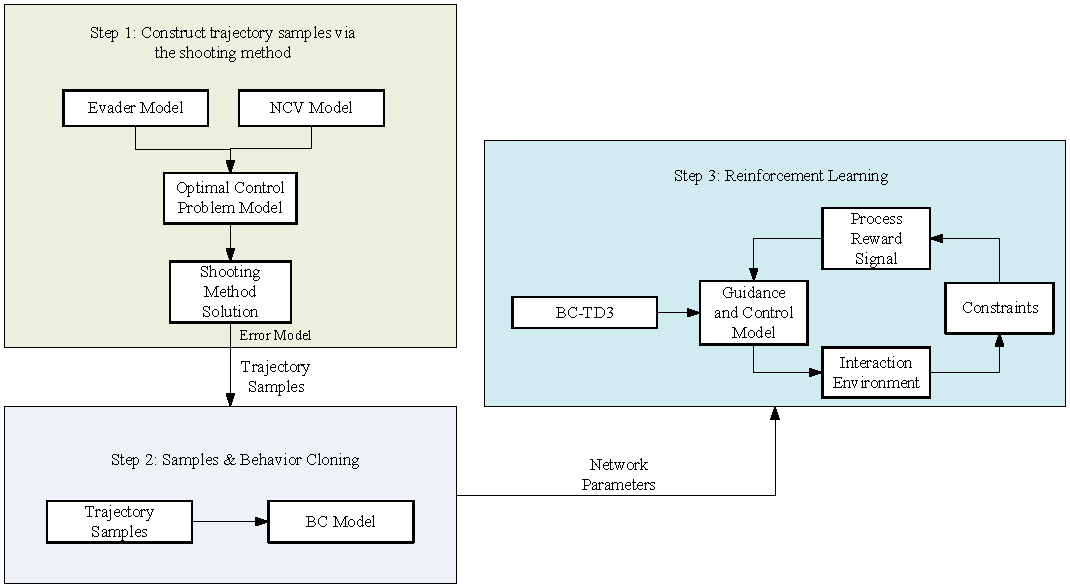
\includegraphics[width=0.82\linewidth]{fig02.pdf}
\caption{BC-TD3 network architecture.}
\label{fig:bctd3-arch}
\end{figure}
The training hyperparameters of BC-TD3 and TD3 are listed in Table~\ref{tab:hyperparams}.

\begin{table}[htbp]
\centering
\caption{Training hyperparameters of TD3 and BC-TD3.}
\label{tab:hyperparams}
\small
\begin{tabularx}{\linewidth}{lXX}
\toprule
Hyperparameter & TD3 & BC-TD3 \\
\midrule
Total training steps & 300 000 & 300 000 \\
Learning rate & 1$\times$$10^{-4}$ & 1$\times$$10^{-4}$ \\
Batch size & 256 & 256 \\
Discount factor $\gamma_{\mathrm{d}}$ & 0.99 & 0.99 \\
Soft-update coefficient $\tau$ & 0.005 & 0.005 \\
Replay capacity & 300 000 & 300 000 \\
Steps before updates & 1 000 & 0 \\
Training frequency & every step & every step \\
Policy delay & 3 & 3 \\
Network structure & [256, 256] & [256, 256] \\
Exploration noise $\sigma$ & 0.1 & 0.1 \\
Target-policy noise & 0.2 & 0.2 \\
Target-noise clip & 0.5 & 0.5 \\
Gradient clip & $\pm$10 & $\pm$10 \\
BC pre-fill ratio & --- & 0.33 \\
Initial BC regularization $\lambda_{\mathrm{BC},0}$ & --- & 1.0 \\
BC regularization decay horizon $K_{\mathrm{BC}}$ & --- & 200 000 steps \\
\bottomrule
\end{tabularx}
\end{table}
\FloatBarrier
\subsubsection{Training of the BC-TD3 network}
The complete offline training procedure is as follows.

\begin{algorithm}[H]
\caption{Offline BC-TD3 training for guidance-parameter optimization}
\label{alg:bctd3}
{\footnotesize
\raggedright
Input: expert data set \(\mathcal{D}_{\text{expert}}\), engagement simulator \(\text{Env}\)\\
Output: trained actor \(\pi_\phi\)\\
// Stage 1: BC pre-training\\
1: Initialize the actor \(\pi_\phi\) with random weights\\
2: for epoch = 1 to \(E_{\text{BC}}\) do\\
3: \quad Sample a minibatch \(\{(\boldsymbol{s}_n, \boldsymbol{a}_n)\}\) from \(\mathcal{D}_{\text{expert}}\)\\
4: \quad Update \(\phi\) by minimizing \(\mathcal{L}_{\text{BC}}\) (\ref{eq:78})\\
5: end for\\
6: Pre-fill the replay buffer \(\mathcal{R}\) with \(\mathcal{D}_{\text{expert}}\)\\
// Stage 2: TD3 fine-tuning\\
7: Initialize the critics \(\psi_1, \psi_2\) and the target networks \(\phi' \leftarrow \phi\), \(\psi_j' \leftarrow \psi_j\)\\
8: for episode = 1 to \(E_{\text{TD3}}\) do\\
9: \quad Reset Env to a random initial condition \(\boldsymbol{s}_0\)\\
10: \quad for \(n = 0, 1, 2, \ldots\) do\\
11: \quad\quad \(\boldsymbol{a}_n = \pi_\phi(\boldsymbol{s}_n) + \boldsymbol{\eta}_n\) \hfill // \ref{eq:84}\\
12: \quad\quad Convert \(\boldsymbol{a}_n\) to \(\boldsymbol{p}_n\), obtain \(\boldsymbol{u}_A^*(t)\) from \eqref{eq:48}, and apply magnitude saturation\\
13: \quad\quad Observe \(\boldsymbol{s}_{n+1}, r_n\) (\ref{eq:74}--\ref{eq:75})\\
14: \quad\quad Store \((\boldsymbol{s}_n, \boldsymbol{a}_n, r_n, \boldsymbol{s}_{n+1})\) in \(\mathcal{R}\)\\
15: \quad\quad Sample a minibatch of \(N\) transitions from \(\mathcal{R}\)\\
16: \quad\quad Compute the target \(y_n\) (\ref{eq:79}--\ref{eq:80})\\
17: \quad\quad Update the critics \(\psi_1, \psi_2\) by minimizing \(\mathcal{L}_{\text{Critic}}\) (\ref{eq:81})\\
18: \quad\quad if \(n \bmod d = 0\) then \hfill // delayed update\\
19: \quad\quad\quad Sample expert pairs, compute \(\lambda_{\mathrm{BC}}(k)\), and update \(\phi\) by minimizing \(\mathcal{L}_{\mathrm{Actor}}\) (\ref{eq:82})\\
20: \quad\quad\quad Soft-update the target networks \(\phi', \psi_j'\) (\ref{eq:83})\\
21: \quad\quad end if\\
22: \quad end for\\
23: end for\\
// Deployment (online inference)\\
24: return \(\pi_\phi\) --- at each guidance cycle, \(\boldsymbol{a} = \pi_\phi(\boldsymbol{s})\), convert it to \(\boldsymbol{p}\), and pass it with the identified matrices to \eqref{eq:48}
}
\end{algorithm}
